%% LyX 2.5.1 created this file.  For more info, see https://www.lyx.org/.
%% Do not edit unless you really know what you are doing.
\documentclass[10pt,english,t,10pt,handout]{beamer}
\usepackage{lmodern}
\usepackage[T1]{fontenc}
\usepackage[utf8]{inputenc}
\setcounter{tocdepth}{1}
\usepackage{bm}
\usepackage{amsbsy}
\usepackage{amstext}
\usepackage{amssymb}
\usepackage[authoryear]{natbib}

\makeatletter
%%%%%%%%%%%%%%%%%%%%%%%%%%%%%% Textclass specific LaTeX commands.
% this default might be overridden by plain title style
\newcommand\makebeamertitle{\frame{\maketitle}}%
% (ERT) argument for the TOC
\AtBeginDocument{%
  \let\origtableofcontents=\tableofcontents
  \def\tableofcontents{\@ifnextchar[{\origtableofcontents}{\gobbletableofcontents}}
  \def\gobbletableofcontents#1{\origtableofcontents}
}

%%%%%%%%%%%%%%%%%%%%%%%%%%%%%% User specified LaTeX commands.



\usepackage{tikz}
\usetikzlibrary{positioning}
\usepackage{appendixnumberbeamer}

\usepackage{graphicx}
\usepackage{subfig}

\usetheme[progressbar=frametitle,block=fill,subsectionpage=progressbar]{metropolis}

% margin
\setbeamersize{text margin right=1.5cm}

% colors
\definecolor{DarkRed}{rgb}{0.7,0,0}
%\colorlet{DarkRed}{red!70!black}
\setbeamercolor{normal text}{fg=black}
\setbeamercolor{alerted text}{fg=DarkRed}
\setbeamercolor{progress bar}{fg=DarkRed}
\setbeamercolor{button}{bg=DarkRed}

% width of seperators
\makeatletter
\setlength{\metropolis@titleseparator@linewidth}{1pt}
\setlength{\metropolis@progressonsectionpage@linewidth}{1pt}
\setlength{\metropolis@progressinheadfoot@linewidth}{1pt}
\makeatother

% new alert block
\newlength\origleftmargini
\setlength\origleftmargini\leftmargini
\setbeamertemplate{itemize/enumerate body begin}{\setlength{\leftmargini}{4mm}}
\let\oldalertblock\alertblock
\let\oldendalertblock\endalertblock
\def\alertblock{\begingroup \setbeamertemplate{itemize/enumerate body begin}{\setlength{\leftmargini}{\origleftmargini}} \oldalertblock}
\def\endalertblock{\oldendalertblock \endgroup}
\setbeamertemplate{mini frame}{}
\setbeamertemplate{mini frame in current section}{}
\setbeamertemplate{mini frame in current subsection}{}
\setbeamercolor{section in head/foot}{fg=normal text.bg, bg=structure.fg}
\setbeamercolor{subsection in head/foot}{fg=normal text.bg, bg=structure.fg}

% footer
\makeatletter
\setbeamertemplate{footline}{%
    \begin{beamercolorbox}[colsep=1.5pt]{upper separation line head}
    \end{beamercolorbox}
    \begin{beamercolorbox}{section in head/foot}
      \vskip1pt\insertsectionnavigationhorizontal{\paperwidth}{}{\hskip0pt plus1filll \insertframenumber{} / \inserttotalframenumber \hskip2pt}\vskip3pt% 
    \end{beamercolorbox}%
    \begin{beamercolorbox}[colsep=1.5pt]{lower separation line head}
    \end{beamercolorbox}
}
\makeatother

% toc
\setbeamertemplate{section in toc}{\hspace*{1em}\inserttocsectionnumber.~\inserttocsection\par}
\setbeamertemplate{subsection in toc}{\hspace*{2em}\inserttocsectionnumber.\inserttocsubsectionnumber.~\inserttocsubsection\par}



% code
\usepackage{xcolor}
\usepackage{listings}

\definecolor{codegray}{rgb}{0.5,0.5,0.5}
\definecolor{background}{HTML}{F5F5F5}
\definecolor{keyword}{HTML}{4B69C6}
\definecolor{string}{HTML}{448C27}
\definecolor{comment}{HTML}{448C27}

\usepackage{inconsolata}
\lstdefinestyle{mystyle}{
    commentstyle=\color{comment},
    keywordstyle=\color{keyword},
    stringstyle=\color{string},
    basicstyle=\ttfamily,
    breakatwhitespace=false,         
    breaklines=true,                 
    captionpos=b,                    
    keepspaces=true,                                    
    numbersep=5pt,                  
    showspaces=false,                
    showstringspaces=false,
    showtabs=false,
    tabsize=4,
	showlines=true
}

\lstset{style=mystyle}
% Added by lyx2lyx
\setlength{\parskip}{\smallskipamount}
\setlength{\parindent}{0pt}

\makeatother

\usepackage{babel}
\begin{document}
\title{13. I-HANK\vspace{-2mm}}
\subtitle{Adv. Macro: Heterogenous Agent Models} 
\author{Raphaël Huleux}
\date{2026}

{
\setbeamertemplate{footline}{} 
\begin{frame}

\maketitle

\end{frame}
}

\addtocounter{framenumber}{-1}

\section{Introduction}
\begin{frame}{Introduction}
\vspace{-2mm}
\begin{itemize}
\item <+->\textbf{So far:}
\begin{itemize}
\item How does heterogeneity matter for business cycles and policy in \textbf{closed
economies}
\end{itemize}
\item <+->\textbf{Today: }
\begin{itemize}
\item Extend to \textbf{small open economy} (SOE) setting 
\item $\Rightarrow$ The \emph{International} HANK Model (\emph{IHANK})
\end{itemize}
\item <+->\textbf{Literature: }
\begin{itemize}
\item {\footnotesize Auclert, Rognlie, Souchier, \& Straub (2024) >>Exchange
rates and monetary policy with heterogeneous agents: Sizing up the
real income channel<<}{\footnotesize\par}
\item {\footnotesize Druedahl, Ravn, Sunder-Plassmann, Sundram, \& Waldstrøm}{\footnotesize\emph{
}}{\footnotesize (2024) >>The Transmission of Foreign Demand Shocks<<}{\footnotesize\par}
\item {\footnotesize Druedahl, Ravn, Sunder-Plassmann, Sundram, \& Waldstrøm}{\footnotesize\emph{
}}{\footnotesize (2024) >>Fiscal Multipliers in Small Open Economies
With Heterogeneous Households<<}{\footnotesize\par}
\end{itemize}
\end{itemize}
\end{frame}
%

\section{IHANK Model }

\begin{frame}{Small Open Economy HANK Model}
\begin{itemize}
\item <+->The >>Small Open economy<< version of the NK model: \textbf{Gali-Monacelli}
(2005) 
\begin{itemize}
\item Adds role for \emph{capital flows, trade} and \emph{exchange rates}
in the NK model 
\end{itemize}
\item <+->IHANK model:
\begin{itemize}
\item Take Gali-Monacelli 
\item Add sticky wages
\item Add heterogeneous agents 
\end{itemize}
\end{itemize}
\end{frame}
%
\begin{frame}{Model components}
\begin{itemize}
\item <+->\textbf{Households}
\begin{itemize}
\item Standard HA: Face idiosyncratic income risk + borrowing constraint 
\item Choose between consumption of domestic and foreign \emph{tradeable}
goods
\end{itemize}
\item <+->\textbf{Firms} 
\begin{itemize}
\item Produce domestic \emph{tradeable} good using labor
\item Have market power 
\end{itemize}
\item <+->\textbf{Unions}
\begin{itemize}
\item Decide on labor supply for HHs subject to wage adjustment cost
\end{itemize}
\item <+->\textbf{Mutual fund}
\begin{itemize}
\item Collect household savings and invest in available assets (domestic
firm equity + \textbf{foreign bonds})
\item $\Rightarrow$ Free capital flows 
\end{itemize}
\item <+->\textbf{Central bank }
\item <+->\textbf{Foreign economy} (mostly exogenous)
\end{itemize}
\end{frame}
%
\begin{frame}{Households}
\begin{itemize}
\item \textbf{Household problem:}
\begin{align*}
v_{t}(z_{it},a_{it-1}) & =\max_{c_{it}}\frac{c^{1-\sigma}_{it}}{1-\sigma}-\varphi\frac{\ell^{1+\nu}_{it}}{1+\nu}+\beta\mathbb{E}_{t}\left[v_{t+1}(z_{it+1},a_{it})\right]\\
\text{s.t. }a_{it}+c_{it} & =(1+r^{a}_{t})a_{t-1}+Z_{t}z_{it}\\
\log z_{it+1} & =\rho_{z}\log z_{it}+\psi_{it+1}\,\,\,,\psi_{t}\sim\mathcal{N}(\mu_{\psi},\sigma_{\psi}),\,\mathbb{E}[z_{it}]=1\\
a_{it} & \geq0
\end{align*}
\item \textbf{Active decisions:} Consumption-saving, $c_{it}$ (and $a_{it}$)
\item \textbf{Union decision:} Labor supply, $\ell_{t}$
\item \textbf{Aggregate Consumption: $C^{hh}_{t}=\int c_{it}d\mathcal{D}_{it}$}
\item \textbf{Consumption function: $C^{hh}_{t}=C^{hh}\left(\{r^{a}_{s},Z_{s}\}^{\infty}_{s=0}\right)$}
\end{itemize}
\end{frame}
%
\begin{frame}{Consumption basket}
\begin{itemize}
\item <+->Consumption $c_{it}$ is a basket composed of:
\begin{itemize}
\item Domestic goods $c_{H,it}$
\item Foreign goods $c_{F,it}$
\end{itemize}
\item <+->CES preferences over these with weight $\alpha$ on imports:
\[
c_{it}=\left[\alpha^{1/\eta}c^{\frac{\eta-1}{\eta}}_{F,it}+\left(1-\alpha\right)^{1/\eta}c^{\frac{\eta-1}{\eta}}_{H,it}\right]^{\frac{\eta}{\eta-1}}
\]
\item <+->\textbf{FOCs}:
\[
c_{F,it}=\alpha\left(\frac{P_{F,t}}{P_{t}}\right)^{-\eta}c_{it},\quad\quad c_{H,it}=\left(1-\alpha\right)\left(\frac{P_{H,t}}{P_{t}}\right)^{-\eta}c_{it},
\]
\item <+->with $P_{t}=$CPI:
\[
P_{t}=\left[\alpha P^{1-\eta}_{F,t}+\left(1-\alpha\right)P^{1-\eta}_{H,t}\right]^{\frac{1}{1-\eta}}
\]
\end{itemize}
\end{frame}
%
\begin{frame}{Aggregate consumption basket }
\begin{itemize}
\item <+->Aggregating we get:
\[
C_{F,t}=\alpha\left(\frac{P_{F,t}}{P_{t}}\right)^{-\eta}C^{hh}_{t},\quad\quad C_{H,t}=\left(1-\alpha\right)\left(\frac{P_{H,t}}{P_{t}}\right)^{-\eta}C^{hh}_{t}
\]
\item <+->Only need aggregate consumption to calculate demand for domestic
and foreign goods
\item <+->Possible because CES preferences are homothetic!
\begin{itemize}
\item All households choose the same consumption basket: $\frac{c_{F,it}}{c_{it}}=\alpha\left(\frac{P_{F,t}}{P_{t}}\right)^{-\eta}$
\end{itemize}
\item <+->If preferences are non-homothetic HH problem is more complicated
\end{itemize}
\end{frame}
%
\begin{frame}{Non-homothetic preferences }
\begin{itemize}
\item <+->If preferences for $\nu\left(c_{F,it},c_{H,it}\right)$ are \textbf{non-homothetic
}rich and poor households will hold different consumption baskets
\item <+->Need to solve more complicated problem (see appendix in Auclert
et al 2024)\\
\begin{align*}
v_{t}(z_{it},a_{it-1}) & =\max_{c_{F,it},c_{H,it}}\nu\left(c_{F,it},c_{H,it}\right)-\varphi\frac{\ell^{1+\nu}_{it}}{1+\nu}+\beta\mathbb{E}_{t}\left[v_{t+1}(z_{it+1},a_{it})\right]\\
\text{\ensuremath{a_{it}}+\ensuremath{\frac{P_{F,t}}{P_{it}}c_{F,it}}} & +\frac{P_{H,t}}{P_{it}}c_{H,it}=(1+r^{a}_{t})a_{t-1}+Z_{t}z_{it}\\
\log z_{it+1} & =\rho_{z}\log z_{it}+\psi_{it+1}\,\,\,,\psi_{t}\sim\mathcal{N}(\mu_{\psi},\sigma_{\psi}),\,\mathbb{E}[z_{it}]=1\\
a_{it} & \geq0
\end{align*}
\item <+->where $P_{it}$ is the ideal price index associated with the
consumption basket of individual $i$
\end{itemize}
\end{frame}
%
\begin{frame}{Prices}
\begin{itemize}
\item <+->In baseline model assume \textbf{law of one price}
\begin{itemize}
\item Prices of the same product are equalized across countries once converted
into same currency
\end{itemize}
\item <+->Implies that the \textbf{price of foreign goods in domestic currency}
$P_{F,t}$ is:
\[
P_{F,t}=P^{\ast}_{F,t}E_{t}
\]
\item <+->where $P^{\ast}_{F,t}$= price of foreign goods in foreign, $E_{t}$=nominal
exchange rate 
\item <+->Note: Usual macro convention, an increase in $E_{t}$ corresponds
to a \textbf{depreciation}
\begin{itemize}
\item So $E_{t}=7,46$ between DKK and EURO for instance
\end{itemize}
\end{itemize}
\end{frame}
%
\begin{frame}{Firms}

\begin{itemize}
\item \textbf{Production and profits:}
\begin{align*}
Y_{t} & =L_{t}\\
\Pi_{t} & =\frac{P_{H,t}}{P_{t}}Y_{t}-\frac{W_{t}}{P_{t}}L_{t}
\end{align*}
\item \textbf{First order condition:}
\[
\frac{P_{H,t}}{P_{t}}\frac{1}{\mu}=w_{t}
\]
\end{itemize}
\end{frame}
%
\begin{frame}{Mutual fund and assets}
\begin{itemize}
\item <+->Mutual fund collect households savings $A_{t}$ 
\item <+->Invest in available assets
\begin{itemize}
\item Firm equity 
\item Foreign bonds $B^{*}_{t}$ (assumption: free capital flows)
\end{itemize}
\item <+->\textbf{Problem}:
\[
\max_{\upsilon_{j,t},B^{*}_{t}}\int\left(\Pi_{j,t+1}+p^{D}_{j,t+1}\right)\upsilon_{j,t}+\frac{\left(1+i^{*}_{t}\right)}{1+\pi_{t+1}}\frac{E_{t+1}}{E_{t}}B^{*}_{t}-\left(1+r^{a}_{t+1}\right)A_{t}
\]
\[
\text{s.t\ensuremath{\quad\int p^{D}_{j,t}\upsilon_{j,t}dj+B^{*}_{t}=A_{t}}}
\]
\item <+->\textbf{FOCs} (no arbitrage conditions):
\begin{align*}
p^{D}_{t} & =\frac{\Pi_{t+1}+p^{D}_{t+1}}{1+r_{t}}\\
1+r_{t} & =\frac{Q_{t+1}}{Q_{t}}\left(1+r^{*}_{t}\right),\quad\quad\text{(UIP)}
\end{align*}
\item <+->\vspace{-0.1cm}where $r_{t}=r^{a}_{t+1}$ the ex-ante interest
rate, $r^{*}_{t}$ is the foreign real interest rate, $Q_{t}=\frac{E_{t}}{P_{t}}P^{*}_{t}$
is the\textbf{ real exchange rate}
\end{itemize}
\end{frame}
%
\begin{frame}{Union}
\begin{itemize}
\item Everybody works the same:
\begin{align*}
\ell_{t} & =L^{hh}_{t}
\end{align*}
\item Maximization subject to wage adjustment cost imply a \textbf{New Keynesian
Wage (Phillips) Curve} (NKWPC or NKWC)
\[
\pi^{w}_{t}=\kappa\left(\varphi\left(L^{hh}_{t}\right)^{\nu}-\frac{1}{\mu}w_{t}\left(C^{hh}_{t}\right)^{\text{-\ensuremath{\sigma}}}\right)+\beta\pi^{w}_{t+1}
\]
\end{itemize}
\end{frame}
%
\begin{frame}{Central bank}
\begin{itemize}
\item <+->\textbf{1.} \textbf{Floating exchange rate:}
\item <+->Will assume float for most of today. Then business as usual:
\[
i_{t}=i_{ss}+\phi\pi_{t},\quad\quad1+r_{t}=\frac{1+i_{t}}{1+\pi_{t+1}}
\]
\item <+->(Note that it might be more suited for CB to target PPI $\pi_{H,t}$)
\item <+->\textbf{2. Fixed exchange rate }

\[
E_{t}=E_{ss}
\]

\item <+->Central bank chooses nominal interest rate such that the nominal
exchange rate is fixed
\item <+->Can also be implemented with a Taylor-type rule:
\[
i_{t}=i_{ss}+\phi_{E}\left(E_{t}-E_{ss}\right)
\]
\item <+->with $\phi_{E}\rightarrow\infty$
\end{itemize}
\end{frame}
%
\begin{frame}{Foreign Economy}
\begin{itemize}
\item <+->Because we focus on a \emph{small open economy }domestic shocks
does not affect the foreign economy
\begin{itemize}
\item Foreign interest rate $r^{*}_{t}$ is exogenous
\item Foreign price $P^{*}_{F,t}$ is exogenous
\end{itemize}
\item <+->Foreign demand for domestic goods given by Armington/CES demand:
\[
C^{\ast}_{H,t}=\alpha\left(\frac{P^{\ast}_{H,t}}{P^{\ast}_{F,t}}\right)^{-\eta^{\ast}}M^{\ast}_{t}
\]
\item <+->where $M^{\ast}_{t}$ is overall demand for foreign goods (shifter)
\item <+->$C^{\ast}_{H,t}$ is overall demand for goods from Home country 
\item <+->Law of one price: $P^{\ast}_{H,t}=\frac{P_{H,t}}{E_{t}}$
\end{itemize}
\end{frame}
%
\begin{frame}{Trade and current account}
\begin{itemize}
\item <+->Define $GDP_{t}=\frac{P_{H,t}}{P_{t}}Y_{t}$. Net exports are:
\[
NX_{t}=GDP_{t}-C^{hh}_{t}
\]
\item <+->The net foreign asset position is
\[
NFA_{t}=A^{hh}_{t}-p^{D}_{t}
\]
\item <+->The current account is:
\[
CA_{t}=NX_{t}+r^{a}_{t}NFA_{t-1}
\]
\item <+->Current account and net foreign asset position are related by
{[}Walras{]}:
\[
NFA_{t}-NFA_{t-1}=CA_{t}
\]
\end{itemize}
\end{frame}
%
\begin{frame}{Market clearing}
\begin{enumerate}
\item Labor market: $L_{t}=L^{hh}_{t}$
\item Goods market (Version 1)
\[
Y_{t}=C_{H,t}+C^{\ast}_{H,t}
\]
\item Goods market (Version 2)
\[
GDP_{t}=C^{hh}_{t}+NX_{t}
\]
\\
with $NX_{t}=\frac{P_{H,t}}{P_{t}}C^{\ast}_{H,t}-\frac{P_{F,t}}{P_{t}}C_{F,t}$
\end{enumerate}
\end{frame}

\section{International Keynesian Cross}
\begin{frame}{Sequence-space - goods market}
\begin{itemize}
\item <+->Linearizing goods mkt' $Y_{t}=C_{H,t}+C^{\ast}_{H,t}$:
\[
d\boldsymbol{Y}=d\boldsymbol{C}_{H}+d\boldsymbol{C}^{\ast}_{H}
\]
\item <+->Linearize CES demand $C_{H,t},C^{\ast}_{H,t}$ around ss:
\begin{align*}
C_{H,t}=\left(1-\alpha\right)\left(\frac{P_{H,t}}{P_{t}}\right)^{-\eta}C^{hh}_{t} & \Rightarrow d\boldsymbol{C}_{H}=\left(1-\alpha\right)d\boldsymbol{C}^{hh}-\eta\left(1-\alpha\right)d\left(\frac{\boldsymbol{P}_{H}}{\boldsymbol{P}}\right)\\
C^{\ast}_{H,t}=\alpha\left(\frac{P^{\ast}_{H,t}}{P^{\ast}_{F,t}}\right)^{-\eta^{\ast}}M^{\ast}_{t} & \Rightarrow d\boldsymbol{C}^{\ast}_{H}=\alpha d\boldsymbol{M}^{\ast}-\eta^{\ast}\alpha d\left(\frac{\boldsymbol{P}^{\ast}_{H}}{\boldsymbol{P}^{\ast}_{F}}\right)
\end{align*}
\item <+->For now assume no change in foreign demand, $d\boldsymbol{M}^{\ast}=0$
\[
d\boldsymbol{Y}=\left(1-\alpha\right)d\boldsymbol{C}^{hh}-\eta\left(1-\alpha\right)d\left(\frac{\boldsymbol{P}_{H}}{\boldsymbol{P}}\right)-\eta^{\ast}\alpha d\left(\frac{\boldsymbol{P}^{\ast}_{H}}{\boldsymbol{P}^{\ast}_{F}}\right)
\]
\end{itemize}
\end{frame}
%
\begin{frame}{Sequence-space - trade elasticity}
\begin{itemize}
\item <+->Linearizing the price index + LOOP gives $dP_{H,t}-dP_{t}=-\frac{\alpha}{1-\alpha}dQ_{t}$
and $dP^{*}_{H,t}=dP_{H,t}-dE_{t}$ to get:
\item <+->so $dP^{*}_{H,t}=dP_{H,t}-dP_{t}-dQ_{t}=-dQ_{t}-\frac{\alpha}{1-\alpha}dQ_{t}=-\frac{1}{1-\alpha}dQ_{t}$
\begin{align*}
d\boldsymbol{Y} & =\left(1-\alpha\right)d\boldsymbol{C}^{hh}+\eta\left(1-\alpha\right)\frac{\alpha}{1-\alpha}dQ_{t}+\eta^{\ast}\frac{\alpha}{1-\alpha}d\boldsymbol{Q}\\
 & =\left(1-\alpha\right)d\boldsymbol{C}^{hh}+\chi\frac{\alpha}{1-\alpha}d\boldsymbol{Q}
\end{align*}
\item <+->with $\chi=\eta\left(1-\alpha\right)+\eta^{\ast}$ being the
\emph{trade elasticity}
\begin{itemize}
\item Captures the elasticity of net exports to changes in relative prices
(the real EXR $Q$)
\item Typically called \emph{expenditure switching }
\item If the DKK appreciates ($d\boldsymbol{Q}\downarrow$) against the
USD both DK HHs and US HHs will \textbf{substitute toward} US goods
($d\boldsymbol{Y}\downarrow$)
\end{itemize}
\end{itemize}
\end{frame}
%
\begin{frame}{Sequence-space - HHs}
\begin{itemize}
\item <+->What can we say about $d\boldsymbol{C}^{hh}$? Consumption function
is $C^{hh}\left(\{r^{a}_{s},Z_{s}\}^{\infty}_{s=0}\right)$:
\[
d\bm{C}^{hh}=\bm{M}^{r^{a}}d\bm{r}^{a}+\bm{M}d\boldsymbol{Z}
\]
\item <+->Use firm FOC + production function $Z_{t}=w_{t}L_{t}=\frac{P_{H,t}}{P_{t}}Y_{t}\Rightarrow dZ_{t}=-\frac{\alpha}{1-\alpha}dQ_{t}+dY_{t}$
+ small valuation effect $\bm{M}^{r^{a}}\approx\bm{M}^{\boldsymbol{r}}$:
\[
d\bm{C}^{hh}=\bm{M}^{\bm{r}}d\bm{r}+\bm{M}d\boldsymbol{Y}-\frac{\alpha}{1-\alpha}\bm{M}d\boldsymbol{Q}
\]
\end{itemize}
\end{frame}
%
\begin{frame}{Sequence-space - Keynesian Cross}
\begin{itemize}
\item <+->Putting it together:
\[
d\bm{Y}\;=\;\underbrace{(1-\alpha)\bm{M}^{r}d\bm{r}}_{\text{1. Interest rate}}\;+\;\underbrace{(1-\alpha)\bm{M}d\bm{Y}}_{\text{2. Multiplier}}\;+\;\underbrace{\chi\frac{\alpha}{1-\alpha}d\bm{Q}}_{\text{3. Exp. switching}}\;-\;\underbrace{\alpha\bm{M}d\bm{Q}}_{\text{4. Real income}}
\]
\end{itemize}
\begin{enumerate}
\item <+->{\footnotesize Standard $r$ effect: Scaled down by $1-\alpha$
since some of domestic demand goes to foreign goods (imports)}{\footnotesize\par}
\item <+->{\footnotesize Standard multiplier: Scales with MPC matrix $\bm{M}$
and home bias $1-\alpha$}{\footnotesize\par}
\item <+->{\footnotesize\textbf{Expenditure switching}}{\footnotesize :
An appreciation of the EXR ($Q\downarrow$) causes substitution away
from home's goods -> less demand for $Y$}{\footnotesize\par}
\item <+->{\footnotesize\textbf{Real income channel of EXR}}{\footnotesize :
Appreciation ($Q\downarrow$) causes foreign goods to be cheaper in
home currency $\Rightarrow$ Reduces $PF,P$, raises real income $Z$}{\footnotesize\par}
\end{enumerate}
\end{frame}

\section{Monetary Policy}
\begin{frame}{Sequence-space - Keynesian Cross}
\begin{itemize}
\item <+->Use the Keynesian Cross to analyze monetary policy with heterogeneous
agents 
\begin{itemize}
\item Reference: {\footnotesize Auclert, Rognlie, Souchier, \& Straub (2024)
>>Exchange rates and monetary policy with heterogeneous agents: Sizing
up the real income channel<<}{\footnotesize\par}
\end{itemize}
\item <+->Fundamental difference in the open economy is that monetary policy
affect EXR through \textbf{UIP:}
\[
1+r_{t}=\frac{Q_{t+1}}{Q_{t}}\left(1+r^{*}\right)
\]
\item <+->For given foreign rate $r^{*}$ an increase in domestic real
rate $r_{t}$ will attract foreign capital flows $\Rightarrow$ Appreciation
of $Q_{t}$ 
\begin{itemize}
\item To first-order we have $dQ_{t}=-\sum^{\infty}_{s\geq t}dr_{s}$ for
a constant $r^{*}$
\end{itemize}
\end{itemize}
\end{frame}
%
\begin{frame}{HANK-RANK equivalence}
\begin{itemize}
\item <+->In closed economy monetary policy was equally effective in HANK/RANK 
\begin{itemize}
\item Under some assumption (log utility, no gov bonds ...)
\end{itemize}
\item <+->Not obvious here since a reduction in $r$ implies a depreciation
which:
\begin{itemize}
\item Decreases demand in HANK due to real income effect 
\item Increases demand for domestic goods through expenditure switching 
\end{itemize}
\item <+->Turns out that these effects \textbf{balance each other exactly}
if trade elasticity $\chi=2-\alpha$
\begin{itemize}
\item If $\chi<2-\alpha$ then the real income effect dominates and monetary
policy \emph{less} effective in HANK
\item If $\chi>2-\alpha$ then expenditure switching dominates and monetary
policy is \emph{more} effective in HANK
\end{itemize}
\end{itemize}
\end{frame}
%
\begin{frame}{Monetary policy - $\chi=2-\alpha$}
\begin{itemize}
\item Output response in HANK/RANK with neutrality, $\chi=2-\alpha$ \vspace{0.5cm}\\
\begin{figure}[H]     
\centering      
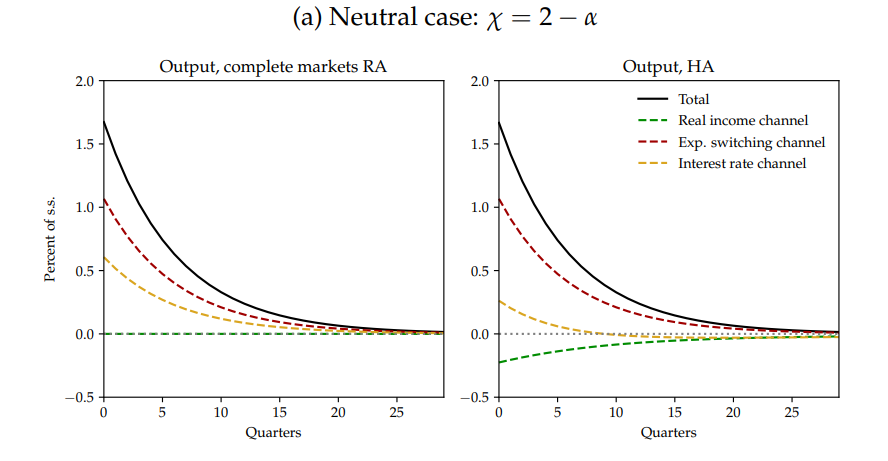
\includegraphics[width=0.9\linewidth]{figs/AMSS2024MonPolNeutral.png}      
\end{figure}
\end{itemize}
\end{frame}
%
\begin{frame}{Monetary policy - $\chi<2-\alpha$}
\begin{itemize}
\item Empirically we expect the trade elasticity to be \textbf{low }in the
short run
\begin{itemize}
\item Takes time for firms/households to respond to changes in relative
prices
\item But \emph{probably} larger in the long run ($\chi>2-\alpha$)
\end{itemize}
\item Output response in HANK/RANK with $\chi=0.5<2-\alpha$
\begin{itemize}
\item Monetary policy \textbf{less} effective in HANK \vspace{0.2cm}\\
\begin{figure}[H]     
\centering      
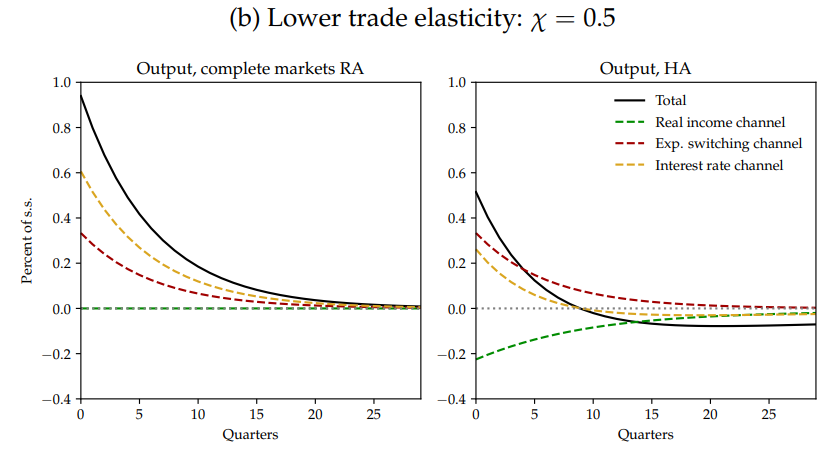
\includegraphics[width=0.8\linewidth]{figs/AMSS2024MonPolLowTrade.png}      
\end{figure}
\end{itemize}
\end{itemize}
\end{frame}

\section{Fiscal Policy}
\begin{frame}{Fiscal Policy}
\begin{itemize}
\item <+->Monetary policy in HANK likely to be \textbf{less effective}
in \textbf{open economy}
\item <+->What about \textbf{fiscal policy?}
\begin{itemize}
\item Recall: In closed economy HANK implied larger fiscal multipliers (/w
deficit financing)
\end{itemize}
\item <+->Take model from before, add government + Taylor rule
\end{itemize}
\end{frame}
%
\begin{frame}{Keynesian cross with G}
\begin{itemize}
\item <+->Keynesian cross:
\begin{align*}
d\bm{Y}\;= & \underbrace{d\bm{G}}_{\text{1. Gov. consumption}}\;-\;\;\underbrace{(1-\alpha)\bm{M}d\bm{T}}_{\text{2. Taxes}}\;+\;\underbrace{(1-\alpha)\bm{M}^{r}d\bm{r}}_{\text{3. Interest rate}}\\
+ & \;\underbrace{(1-\alpha)\bm{M}d\bm{Y}}_{\text{4. Multiplier}}\;+\;\underbrace{\chi\frac{\alpha}{1-\alpha}d\bm{Q}}_{\text{5. Exp. switching}}\;-\;\underbrace{\alpha\bm{M}d\bm{Q}}_{\text{6. Real income}}
\end{align*}
\item <+->Note, with a constant $r$-rule, $d\boldsymbol{r}=0$ this \emph{almost}
reverts to closed economy Cross:
\[
d\bm{Y}=d\bm{G}-(1-\alpha)\bm{M}d\bm{T}+(1-\alpha)\bm{M}d\bm{Y}
\]
\item <+->In fact \textbf{isomorphic} to closed economy Cross with $\bm{\tilde{M}}\equiv(1-\alpha)\bm{M}$
\[
d\bm{Y}=d\bm{G}-\bm{\tilde{M}}d\bm{T}+\bm{\tilde{M}}d\bm{Y}
\]
\end{itemize}
\end{frame}
%
\begin{frame}{Fiscal policy in the open economy}
\begin{itemize}
\item <+->Do we expect fiscal policy to be more or less effective in HANK
vs. RANK?
\item <+->\textbf{More effective:}
\begin{itemize}
\item Positive spending shock $d\boldsymbol{G}>0$ forces CB to raise $\boldsymbol{r}$
implying an appreciation ($d\boldsymbol{Q}$<0)
\item Foreign goods become cheaper, raises real income $\Rightarrow$ More
demand 
\end{itemize}
\item <+->\textbf{Less effective:}
\begin{itemize}
\item Appreciation of EXR implies expenditure switching, so drop in NX
\item Multiplier effect $\bm{M}d\bm{Y}$ is weaker in SOE since a share
$\alpha$ is spend on foreign goods
\end{itemize}
\item <+->Ultimately, a \textbf{quantitative} \textbf{question}
\item <+->... but some analytical results in paper, for instance:
\begin{itemize}
\item In limit $\alpha\rightarrow1$ (fully open economy) HANK/RANK equivalence
since multiplier effects do not matter
\end{itemize}
\end{itemize}
\end{frame}
%
\begin{frame}{Fiscal spending shocks}
\begin{itemize}
\item Main result with deficit financed G shock:\\
\begin{figure}[H]     
\centering      
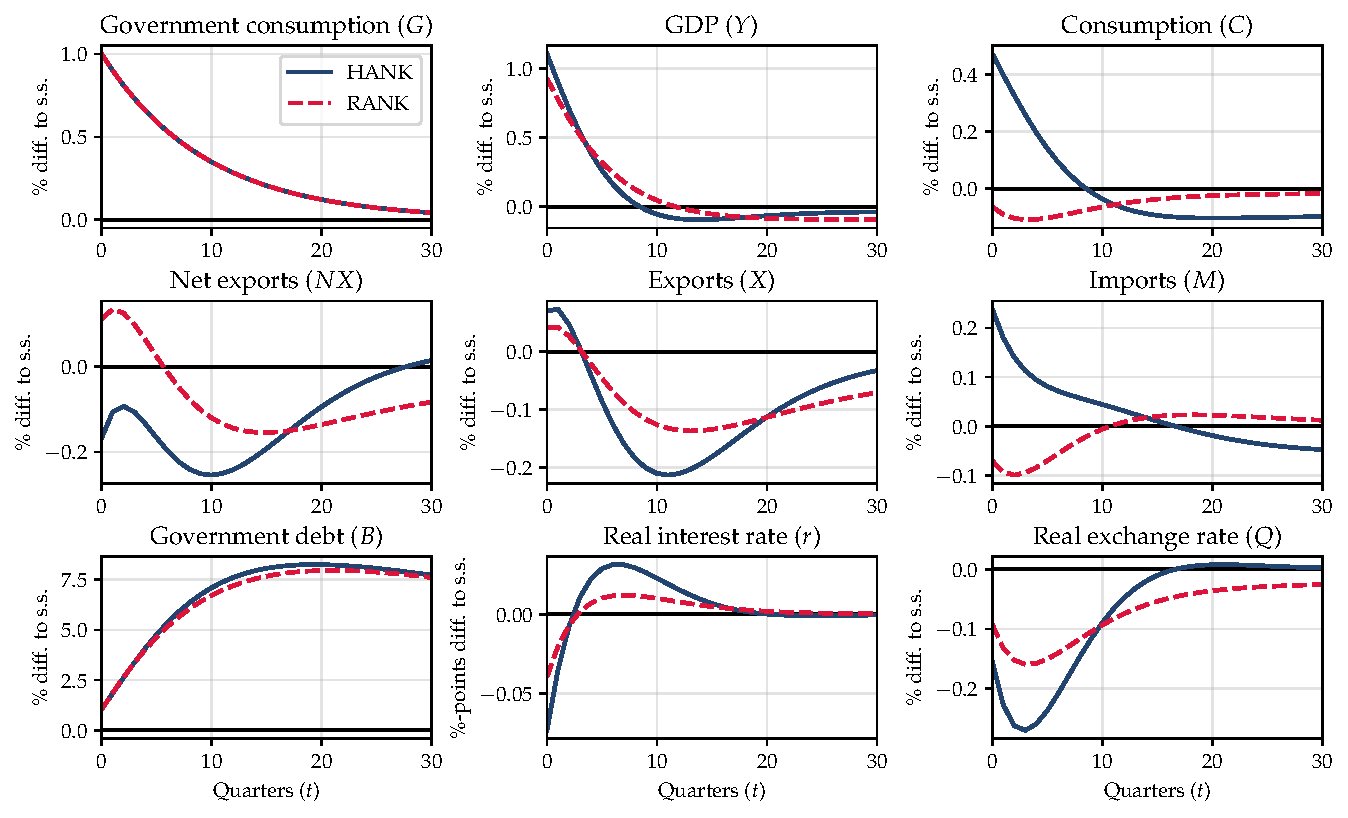
\includegraphics[width=0.8\linewidth]{figs/FiscalIHANKMain.pdf}      
\end{figure}
\item Relatively similar fiscal multiplier
\begin{itemize}
\item HANK produces \textbf{much }larger C response
\item ... But this gets counteracted by larger drop in net exports
\end{itemize}
\end{itemize}
\end{frame}
%
\begin{frame}{Fiscal spending shocks - openness}
\begin{itemize}
\item How does fiscal multiplier vary with openness $\alpha$? (plot IRFs
for first and third quartile of $\frac{Imports}{GDP}$ across sample
of OECD countries.)\\
\begin{figure}[H]     
\centering      
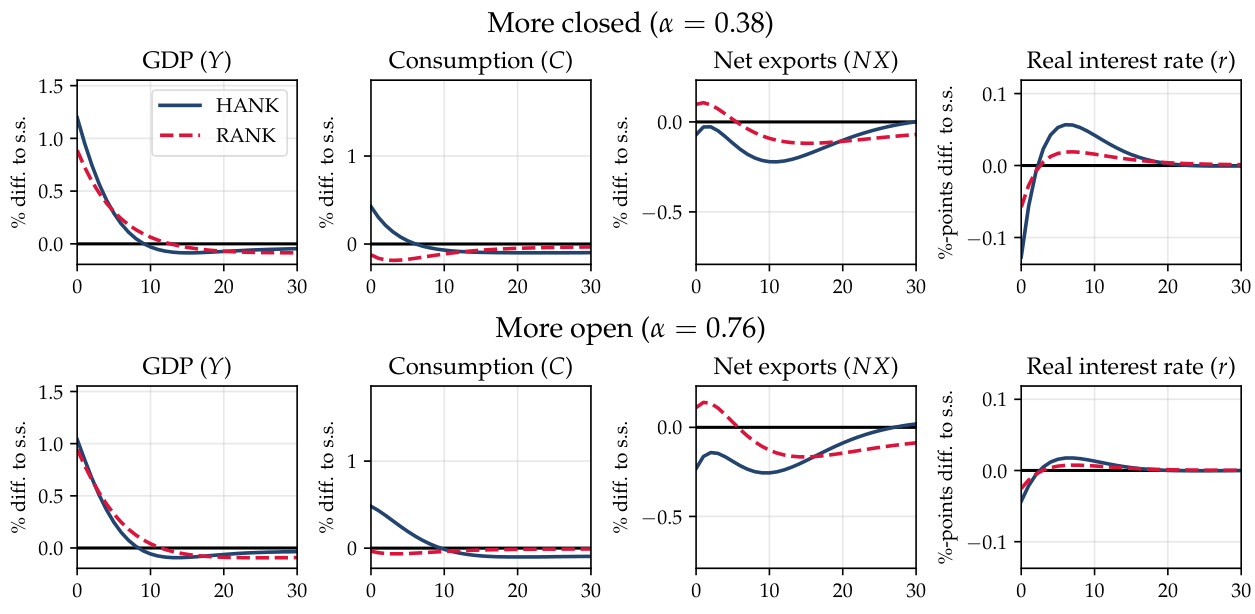
\includegraphics[width=0.9\linewidth]{figs/FiscalPolAlpha.png}      
\end{figure}
\end{itemize}
\end{frame}

\section{Foreign Demand Shocks}
\begin{frame}{Foreign Demand Shocks}
\begin{itemize}
\item <+->So far: How HANK affects transmission of \textbf{policy}
\item <+->Now: How does HANK affect transmission of \textbf{shocks/disurbances}?
\item <+->Focus on a shock to \textbf{foreign demand for domestic goods}
\begin{itemize}
\item <+->E.g. how does a recession in germany affect Denmark via trade
spillovers?
\item <+->Turns out to have important implications for transmission with
HA as opposed to RA
\item <+->Main ref: Druedahl, Ravn, Sunder-Plassmann, Sundram, \& Waldstrøm\emph{
}(2024) >>The Transmission of Foreign Demand Shocks<<
\end{itemize}
\item <+->Other shocks often studied in open economy context:
\begin{itemize}
\item Foreign monetary policy shocks
\item Capital flow shocks (>>sudden stops<<)
\item Import price shocks
\end{itemize}
\end{itemize}
\end{frame}
%
\begin{frame}{Motivaton}
\begin{itemize}
\item <+->Motivation: Go back to international Kenyesian Cross with foreign
demand $\boldsymbol{M}^{*}$
\[
d\bm{Y}=(1-\alpha)\bm{M}^{r}d\bm{r}+(1-\alpha)\bm{M}d\bm{Y}+\chi\frac{\alpha}{1-\alpha}d\bm{Q}-\alpha\bm{M}d\bm{Q}+\alpha d\boldsymbol{M}^{\ast}
\]
\item <+->Can solve this for response of $\boldsymbol{C}$ (see appendix):
\[
d\bm{C}=\Big[\underbrace{\bm{M}}_{\text{Labor income (\ensuremath{>0})}}+\underbrace{\frac{\alpha}{1-\alpha}\bm{M}\bm{G}^{Q,Y}}_{\text{Real income of EXR (\ensuremath{\lessgtr0})}}+\underbrace{\bm{M}^{r}\bm{G}^{r,Q}\bm{G}^{Q,Y}}_{\text{Intertemporal sub. (\ensuremath{<0})}}\Big]\mathcal{M}d\bm{M^{\ast}}
\]
\item <+->RANK with $\bm{M}\approx0$ predicts $d\bm{C}>0$ in response
to a negative foreign demand shock $d\bm{M^{\ast}}<0$
\item <+->HANK can potentially get $d\bm{C}<0$ (\textbf{co-movement})
if labor income channel is strong enough
\item <+->What is sign of $cov\left(d\bm{C},d\bm{M^{\ast}}\right)$ empirically?
\end{itemize}
\end{frame}
%
\begin{frame}{Empirical estimates of foreign demand shock}
\begin{itemize}
\item <+->Panel of 38 OECD contries, focus on 31 SOE's 
\item <+->Trade-weighted country $i$ specific \textquotedbl foreign economy\textquotedbl{}
$(Y^{*}_{i,t},\pi^{*}_{i,t},i^{*}_{i,t})$
\item <+->Use \emph{sign-restrictions} to get foreign demand shock 
\begin{itemize}
\item $dY^{*}_{i,t},d\pi^{*}_{i,t},di^{*}_{i,t}$ all have same sign in
first year
\end{itemize}
\item <+->Estimated foreign shock\vspace{0.5cm}\\
\begin{figure}[H]     
\centering      
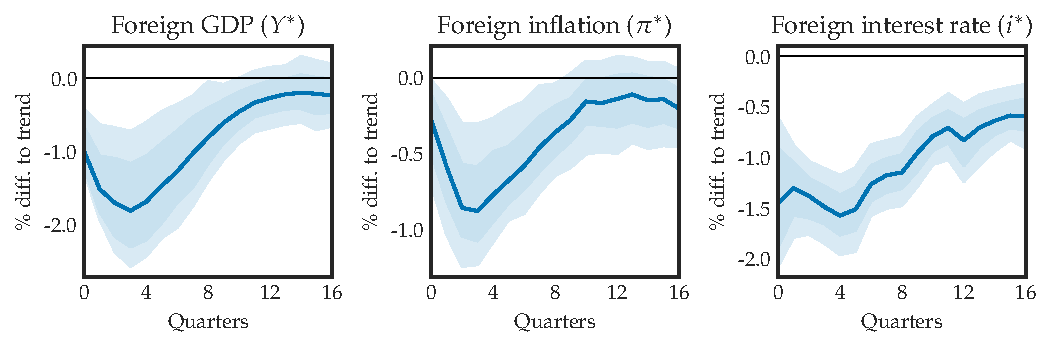
\includegraphics[width=0.9\linewidth]{figs/fig_large.pdf}      
\end{figure}
\end{itemize}
\end{frame}
%
\begin{frame}{Spillover effects}
\begin{itemize}
\item Use estimated shock in foreign trading parters to estimate effects
on domestic, SOE economy
\item Estimate dyanmic OLS/LP $y_{c,t+h}=\beta_{h}i^{*}_{c,t}+\alpha_{h}\pi^{*}_{c,t}+\Theta_{h}M^{*}_{c,t}$
where $y$ = domestic outcomes (GDP,C ...) \\
\begin{figure}[H]     
\centering      
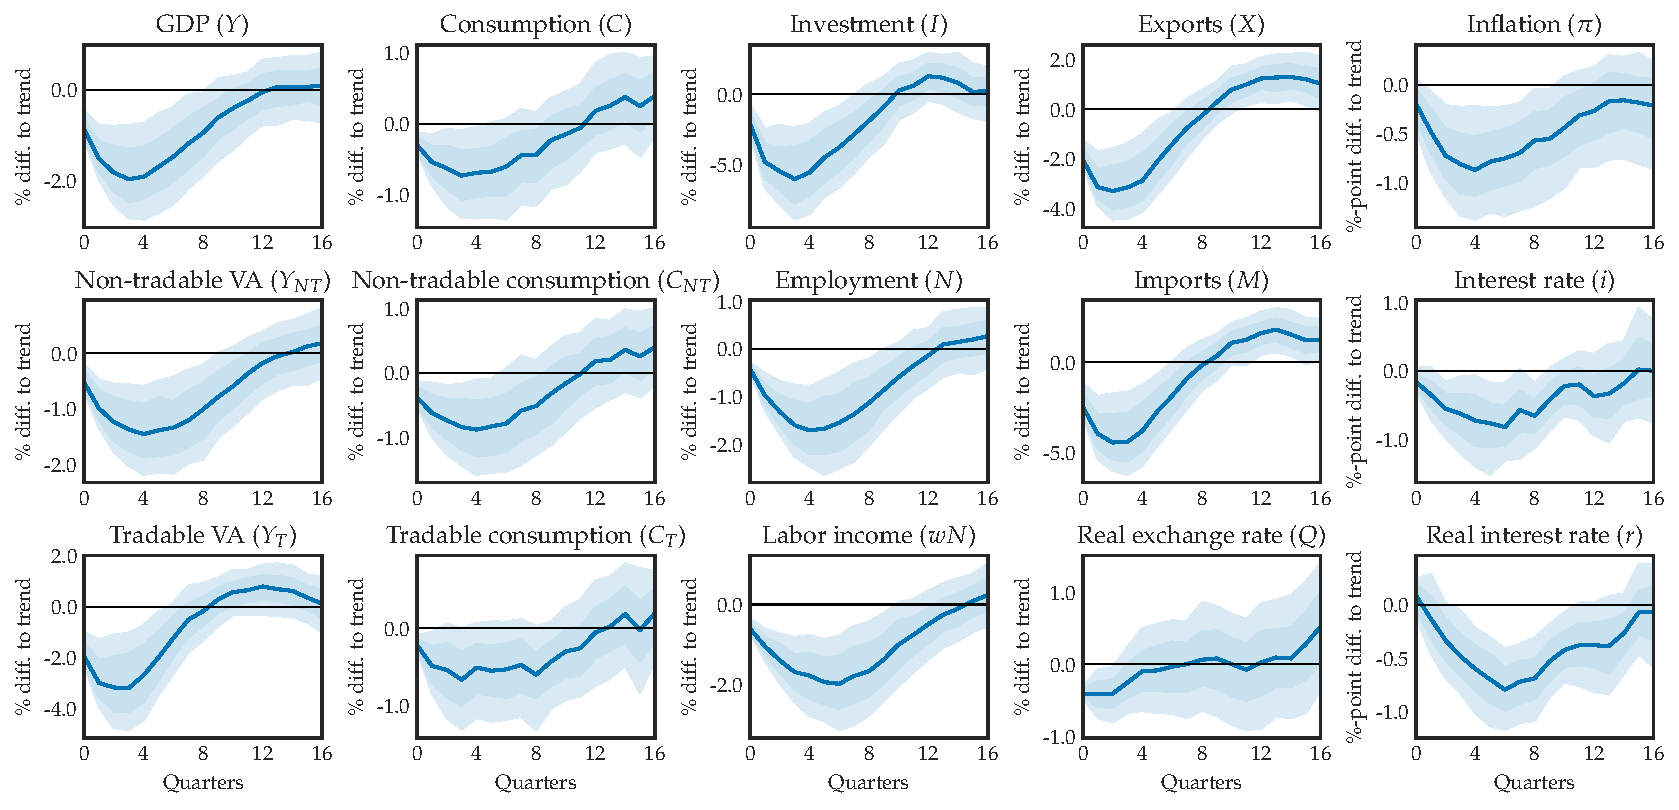
\includegraphics[width=0.9\linewidth]{figs/fig_main.pdf}      
\end{figure}
\end{itemize}
\end{frame}
%
\begin{frame}{Why foreign demand shocks?}
\begin{itemize}
\item <+->Why focus specifically on a \textbf{foreign demand shock?}
\begin{itemize}
\item Provides very clean testable implications for HANK and RANK
\item domestic $r$ increases in response to $d\boldsymbol{M}^{*}<0$
\item Almost always the case since monetary policy does not face output/inflation
tradeoff with demand shock
\end{itemize}
\item <+->Not true for foreign monetary policy shock or supply shock
\item <+->What about domestic demand shock (G)?
\begin{itemize}
\item Identification more difficult 
\item Literature ambiguous on whether C increases or decreases 
\end{itemize}
\end{itemize}
\end{frame}
%
\begin{frame}{Model}
\begin{itemize}
\item <+->\textbf{Next}: Go to medium scale HANK model to see if we can
replicate empirical evidence
\item <+->Model features:
\begin{itemize}
\item Two sectors (tradeable and non-tradeables) + input-output production
structure
\item Government
\item Sticky prices and wages 
\item Dynamic trade elasticities 
\end{itemize}
\item <+->Feed in estimated foreign demand shock, compare with empirics
\end{itemize}
\end{frame}
%
\begin{frame}{Household block}
\begin{itemize}
\item <+->Household problem:
\begin{alignat*}{1}
V_{t}(e_{t},a_{t-1},\beta,s) & =\max_{c_{t},a_{t}}\frac{c^{1-\sigma}_{t}}{1-\sigma}-\nu\frac{L^{1+\frac{1}{\varphi}}_{s,t}}{1+\frac{1}{\varphi}}+\beta_{t}\mathbb{E}_{t}\left[V_{t+1}(e_{t+1},a_{t},\beta,s)\right]\\
 & \text{s.t.}\\
c_{t}+a_{t} & =\left(1+r^{a}_{t}\right)a_{t-1}+\left(1-\tau_{t}\right)w_{s,t}L_{s,t}e_{t}+T_{t}\\
a_{t} & \geq0\\
\ln e_{t} & =\rho_{e}\ln e_{t-1}+\epsilon^{e}_{t},\quad\epsilon^{e}_{t}\sim\mathcal{N}\left(0,\sigma^{2}_{e}\right)
\end{alignat*}
\item <+->Markov matrix for $s$ is $P^{s}=\left[\begin{array}{cc}
1 & 0\\
0 & 1
\end{array}\right]$
\begin{itemize}
\item HHs cannot move sectors. Harsh assumption, but consistent with short-run
dynamics. Can alleviate by changing $P^{s}$ 
\item Could also have endogoues sector choice at HH level 
\end{itemize}
\end{itemize}
\end{frame}
%
\begin{frame}{Model fit - floating}
\begin{itemize}
\item Effects of foreign demand shock with a floating EXR\vspace{1cm}\\
\begin{figure}[H]     
\centering      
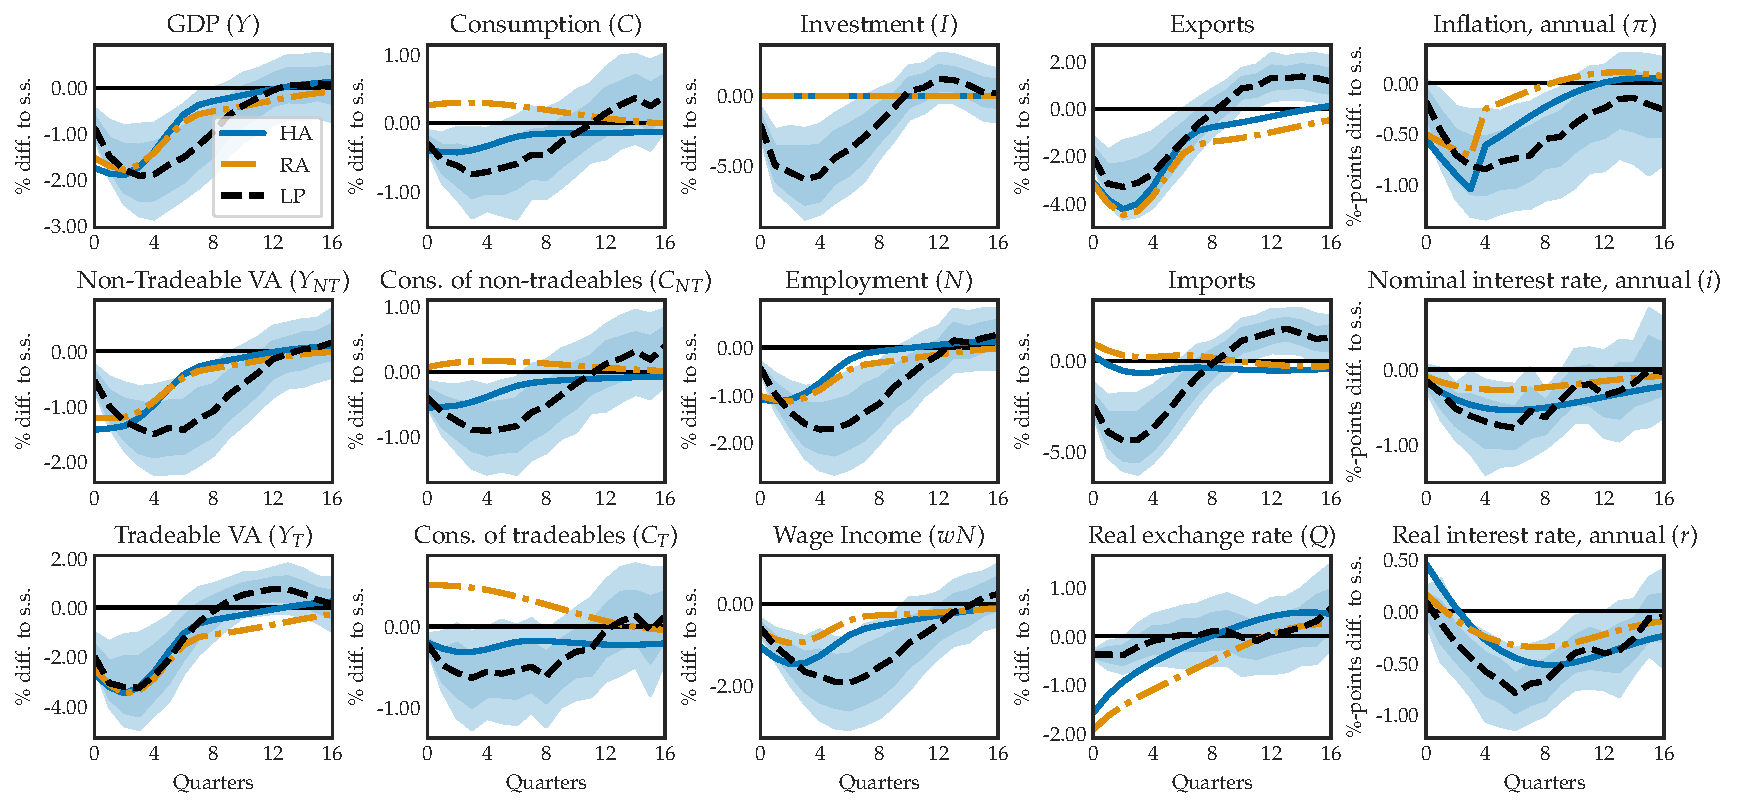
\includegraphics[width=0.95\linewidth]{figs/responses_no_capital_floating.pdf}      
\end{figure}
\end{itemize}
\end{frame}
%
\begin{frame}{Decomposition}
\begin{itemize}
\item Decompose $d\boldsymbol{C}$ into effects from interest rate, labor
income and capital gain effects\\
\begin{figure}[H]     
\centering      
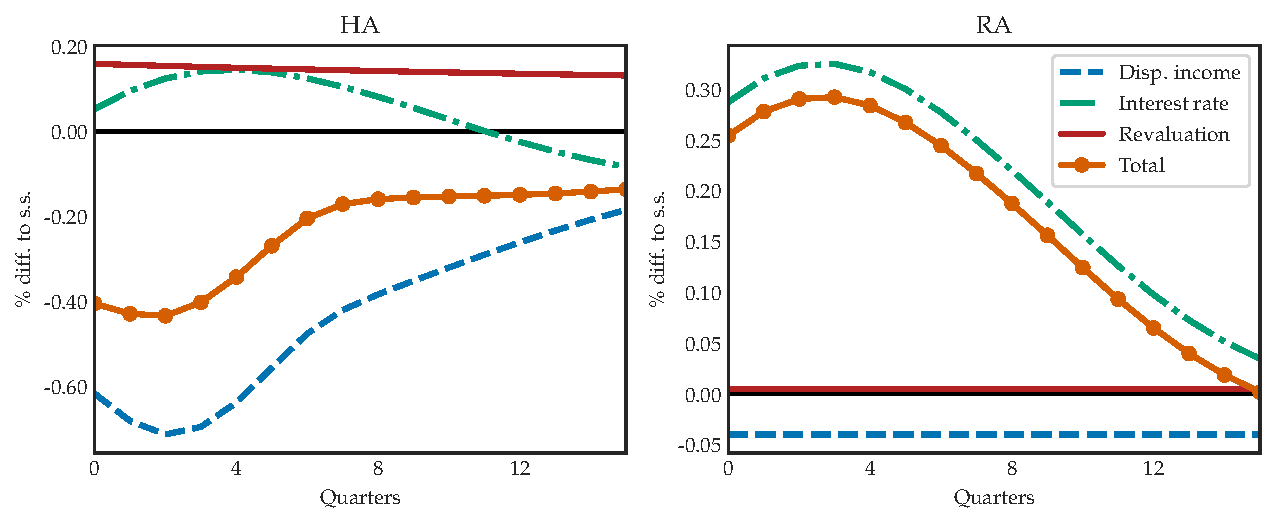
\includegraphics[width=0.9\linewidth]{figs/decomp_no_capital_floating.pdf}      
\end{figure} 
\end{itemize}
\end{frame}
%
\begin{frame}{Model fit - floating /w investment}
\begin{itemize}
\item HANK response amplified by investment
\item Note: Getting investment response right requires exogenous shock to
investment\\
\begin{figure}[H]     
\centering      
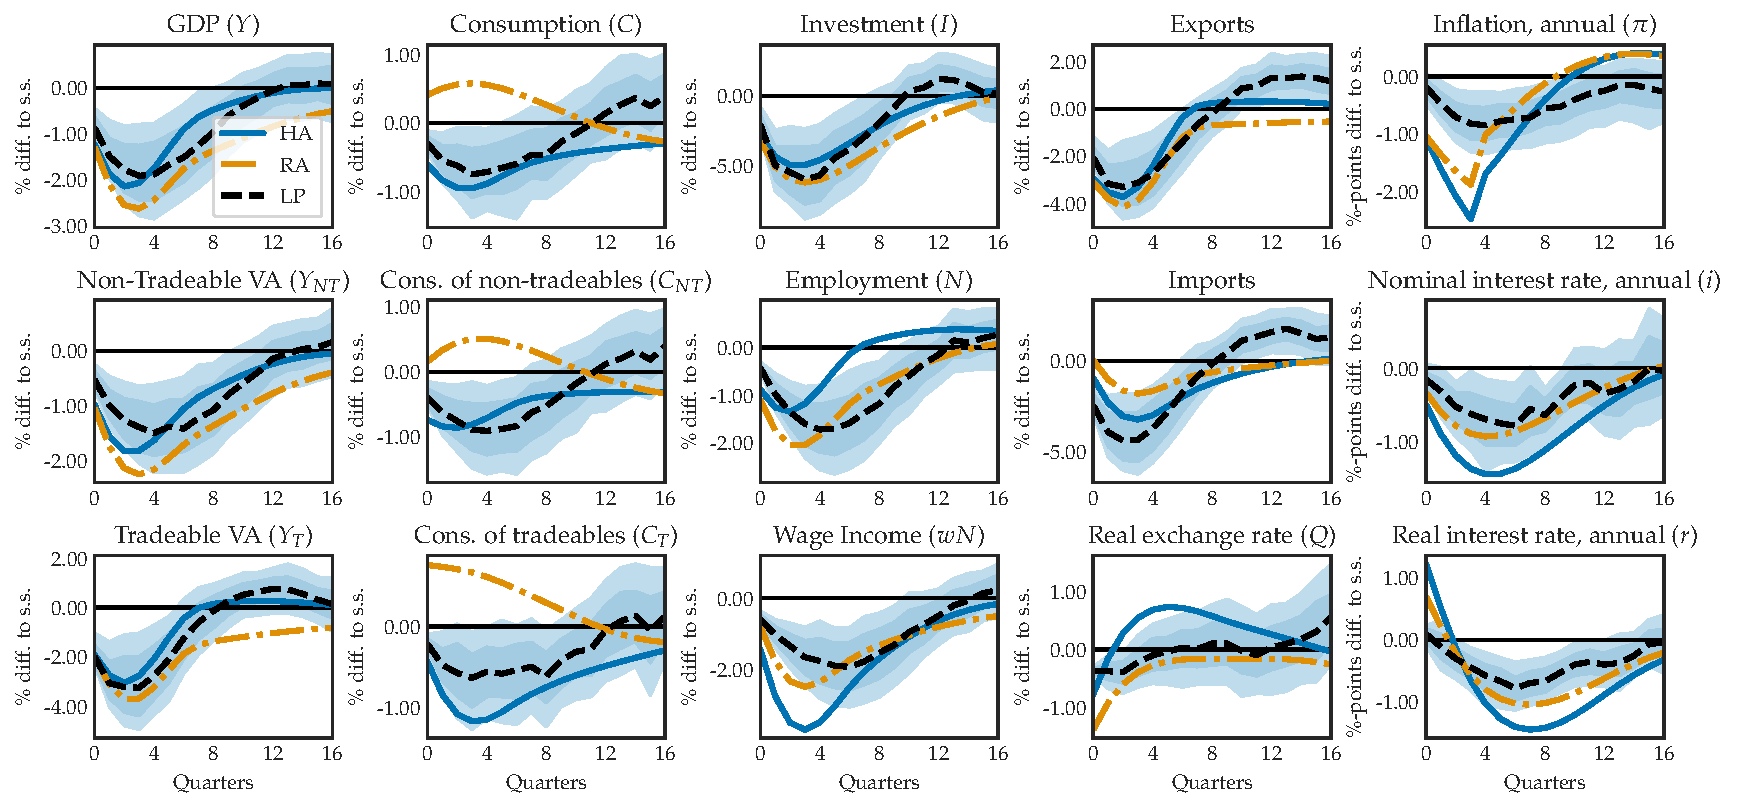
\includegraphics[width=0.9\linewidth]{figs/responses_floating.pdf}      
\end{figure}
\end{itemize}
\end{frame}
%
\begin{frame}{Fixed exchange rate}
\begin{itemize}
\item <+->The Taylor rule is crucial to obtain $i_t \downarrow$, $r_t \downarrow$,
and $C_t \uparrow$ in RANK
\item <+->Does this mean that our result changes under a fixed exchange
rate?
\item <+->\textbf{No}! UIP condition + Fisher equation: 
\begin{alignat*}{1}
1+i_{t}=1+i^{*}_{t}\quad & \Leftrightarrow\quad1+r_{t}=\frac{1+i^{*}_{t}}{1+\pi_{t+1}}
\end{alignat*}
\item <+->A foreign demand shock entails a decline in $i_t^*$ (in both
model and data). 
\item <+->UIP forces central bank in SOE to reduce $i_t$, so $r_t \downarrow$ (unless $\pi_{t+1} \downarrow \downarrow$)
\end{itemize}
\end{frame}
%
\begin{frame}{Model fit - fixed}
\begin{itemize}
\item Similar outcomes with fixed EXR \vspace{0.5cm}\\
\begin{figure}[H]     
\centering      
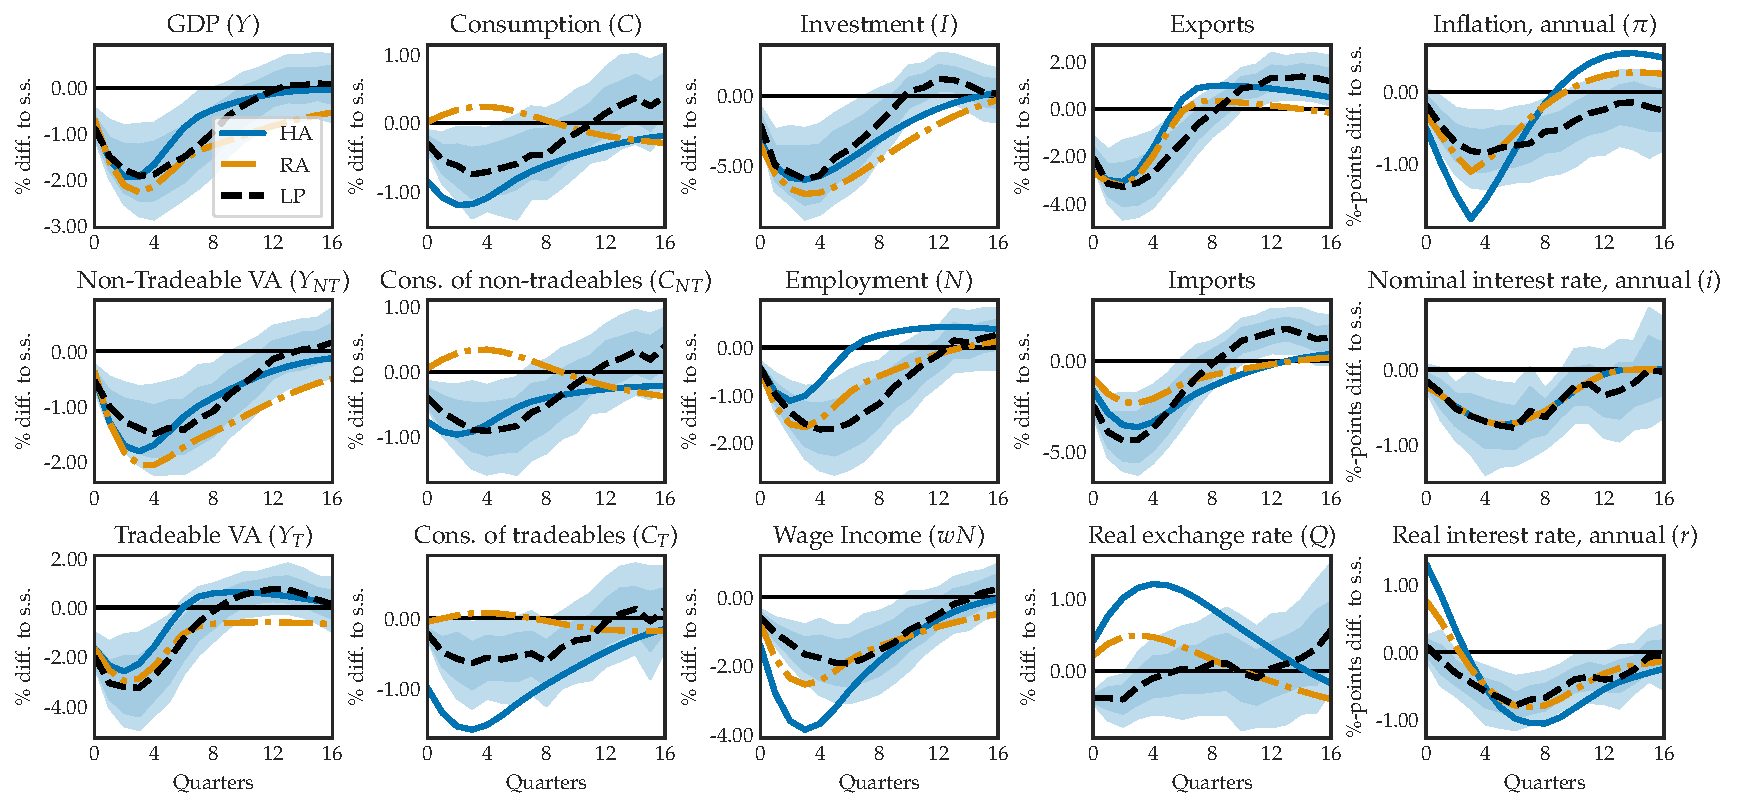
\includegraphics[width=0.9\linewidth]{figs/responses_fixed.pdf}      
\end{figure}
\end{itemize}
\end{frame}
%
\begin{frame}{Policy}
\begin{itemize}
\item <+->Foreign demand shock implies domestic recession for HHs in all
sectors $\Rightarrow$ Welfare loss 
\item <+->Exercise: Calibrate policy shocks (monetary and fiscal policy
seperatly) to stabilize agg. $C$ following foreign demand shock \begin{table}[H]         \centering         
\begin{tabular}{lrrr}         \hline\hline                            & $C$     & $C_T^{hh}$ & $C_{NT}^{hh}$ \\         \hline          
Foreign demand     & $-1.00$ & $-1.27$    & $-0.91$ \\         
Public consumption & $1.00$  & $0.08$     & $1.32$ \\         
Monetary policy    & $1.00$  & $1.01$     & $1.00$ \\         \hline\hline          
\end{tabular}     \end{table}
\item <+->Monetary policy has symmetric effects across sectors $\Rightarrow$
Well suited here
\item <+->Fiscal policy loads on NT sector $\Rightarrow$ Very asymmetric
effects, barely helps HHs in T sector
\begin{itemize}
\item Issues for countries fixed EXRs or in monetary unions 
\item Need targeted transfers
\end{itemize}
\end{itemize}
\end{frame}
%
\begin{frame}{Conclusion}
\begin{itemize}
\item How does heterogeneity affect transmission of shocks and policies
in SOEs?
\begin{itemize}
\item Monetary policy - Likely to be less effective due to real income channel
of EXR
\item Fiscal policy - Closer to RANK multipliers due to crowding out of
NX
\item Foreign demand shocks - larger transmission to domestic spending 
\end{itemize}
\end{itemize}
\end{frame}
%
\begin{frame}{IHANK - litterature}
\begin{itemize}
\item Covered 3 papers here: Other papers in the litterature on HANK in
open economies include:
\end{itemize}
\begin{enumerate}
\item {\footnotesize Guo, X., Ottonello, P., \& Perez, D. J. (2023) }{\footnotesize\emph{Monetary
policy and redistribution in open economies}}{\footnotesize\par}
\begin{itemize}
\item {\footnotesize Redistributional effects of monetary policy in SOEs}{\footnotesize\par}
\end{itemize}
\item {\footnotesize Aggarwal, R., Auclert, A., Rognlie, M., \& Straub, L.
(2023). }{\footnotesize\emph{Excess savings and twin deficits: The
transmission of fiscal stimulus in open economies}}{\footnotesize\par}
\begin{itemize}
\item {\footnotesize Fiscal stimulus in a multi-country model }{\footnotesize\par}
\end{itemize}
\item {\footnotesize De Ferra, S., Mitman, K., \& Romei, F. (2020). }{\footnotesize\emph{Household
heterogeneity and the transmission of foreign shocks}}{\footnotesize{} }{\footnotesize\par}
\begin{itemize}
\item {\footnotesize Effects of exchange rate depreciations when HHs have
foreign currency debt }{\footnotesize\par}
\end{itemize}
\item {\footnotesize Bayer, C., Kriwoluzky, A., Müller, G. J., \& Seyrich,
F. (2024). }{\footnotesize\emph{A HANK$^{2}$ model of monetary unions}}{\footnotesize .
Journal of Monetary Economics }{\footnotesize\par}
\begin{itemize}
\item {\footnotesize A 2-country HANK model}{\footnotesize\par}
\end{itemize}
\end{enumerate}
\end{frame}
%

\section{Summary}
\begin{frame}{Summary and next week}
\begin{itemize}
\item \textbf{Today: }Small open economy HANK models
\item \textbf{Next week: }
\begin{itemize}
\item Advanced HANK topics (\textbf{research frontier})
\item Q\&A
\item Exam
\end{itemize}
\item \textbf{Homework:}
\begin{enumerate}
\item Work on assignment 
\end{enumerate}
\end{itemize}
\end{frame}
%

\end{document}
